\documentclass[xetex,xcolor={table,usenames,dvipsnames}]{beamer}
\usepackage{ragged2e} % Ensure ragged2e is included
\usepackage{beamerthemesplit}
\usepackage[utf8]{inputenc}
\usepackage[T1]{fontenc}
\usepackage[english,french]{babel}
\usepackage{times}
\usepackage{tabularx}
\usepackage{dsfont}
\usepackage{textcomp}
\usepackage{amssymb}
\usepackage{graphicx}
\usepackage{bbding}
\usepackage[absolute,overlay]{textpos}
\usepackage[style=authoryear, maxbibnames=99, mincitenames=1, maxcitenames=2, backref=true, hyperref=true, dashed=false, firstinits=true, backend=bibtex, bibencoding=utf8, uniquename=false, uniquelist=false, natbib=true]{biblatex}
\renewcommand*{\bibfont}{\scriptsize}
\setbeamerfont{footnote}{size=\tiny}

% Remove quotation marks from titles
\DeclareFieldFormat[article,incollection,inproceedings,conference]{title}{#1} 

\usepackage{makecell}

\usepackage{capt-of}

\usepackage{xcolor}
\usepackage{shadowtext} 
% Define a custom color for lavender
\definecolor{lavender}{RGB}{230,230,250}


\usepackage{hyperref}
 
 \hypersetup{
    colorlinks=true,      % Enable colored links
   linkcolor=violet,        % Color for internal links (sections, equations, etc.)
    citecolor=BlueViolet,      % Color for citations
    filecolor=magenta,    % Color for file links
    urlcolor=blue         % Color for URLs
}

\mode<presentation>
{
\usetheme{metropolis}


\setbeamercolor{header}{bg=MidnightBlue, fg=white} % Dark theme header
\setbeamercolor{progressdots}{fg=white} % Color for navigation dots

\setbeamertemplate{headline}{%
	% First row: Section Titles
	\begin{beamercolorbox}[wd=\paperwidth,ht=2.5ex,dp=1ex,center]{header}
		\textbf{\insertsectionnavigationhorizontal{\paperwidth}{}{}}
	\end{beamercolorbox}
	
	% Second row: Navigation Dots (one per frame under each section)
	\begin{beamercolorbox}[wd=\paperwidth,ht=1.5ex,dp=0ex,center]{progressdots}
		\hspace{5pt} % Adjust spacing
		\foreach \sec in \inserttotalsections { % Loop through sections
			\foreach \fr in {1,...,\insertsectionframe} { % Loop through frames in section
				\ifnum\fr=\insertframeinsection
				{\color{white}●} % Highlight current frame in section
				\else
				{\color{gray}○} % Other frames in section
				\fi
				\hspace{3pt} % Adjust spacing between dots
			}
			\hspace{10pt} % Space between sections
		}
	\end{beamercolorbox}
}

\setbeamertemplate{footline}{%
	\begin{beamercolorbox}[wd=\paperwidth,ht=2.5ex,dp=1ex,leftskip=3mm,rightskip=3mm]{footline}
		\hspace{3mm} \textbf{Ljudmila PETKOVI\'C} \hfill
		\textbf{\textsc{M2SOL034} : Introduction, notions de base et aperçu du cours} \hfill
		\textbf{\today} \hspace{3mm}
	\end{beamercolorbox}%
}

\setbeamertemplate{headline}{%
	\begin{beamercolorbox}[wd=\paperwidth,ht=2ex,dp=1ex,center]{frametitle}
		\insertsectionnavigationhorizontal{\paperwidth}{}{}
	\end{beamercolorbox}%
}
\setbeamertemplate{footline}{%
	\begin{beamercolorbox}[wd=\paperwidth,ht=4ex,dp=1ex,leftskip=3mm,rightskip=3mm]{footline}
		\hspace{3mm} 
		\textcolor{gray}{\textbf{Ljudmila PETKOVI\'C}} \hfill
		\textcolor{gray}{\textbf{\textsc{M2SOL034} : Introduction, notions de base et aperçu du cours}} \hfill 
		\textcolor{gray}{\textbf{\today}} \hspace{3mm}
		\textcolor{gray}{\textbf{\insertframenumber{} / \inserttotalframenumber}} \hspace{3mm} % Page number in bottom-right
	\end{beamercolorbox}%
	
	% Add the logo only if we're NOT on the title slide
	\ifnum\insertframenumber>0
	\begin{textblock*}{2.5cm}(\paperwidth-2cm,1\textheight) % Move slightly down and right
		
\includegraphics[width=1.2cm]{img/logo.png} % Adjusted logo size
	\end{textblock*}
	\fi
}









%\usecolortheme{beaver}
\usefonttheme{professionalfonts}
}







\usepackage{listings}

\lstset{ 
  language=C,                     % Set language
  basicstyle=\ttfamily\small,      % Set basic style to small monospaced font
  keywordstyle=\color{blue},       % Set keywords in blue
  commentstyle=\color{gray},       % Set comments in gray
  stringstyle=\color{red},         % Set strings in red
  numbers=left,                    % Line numbers on the left
  numberstyle=\tiny\color{gray},   % Style for line numbers
  stepnumber=1,                    % Line number step
  showstringspaces=false,          % Don't show spaces in strings
  tabsize=4,                       % Set tab size
  breaklines=true,                 % Break long lines
  captionpos=b                     % Caption position bottom
}

\usepackage[font=scriptsize,justification=centering]{caption}
\setbeamercolor{normal text}{fg=black,bg=black}
\setbeamercolor{frametitle}{fg=purple,bg=white}
\setbeamercolor{background canvas}{bg=white}
\setbeamercolor{title}{fg=purple}
\setbeamercolor{subtitle}{fg=purple}
\setbeamercolor{section in toc}{fg=purple}
\setbeamercolor{footline}{fg=purple,bg=white}
%\setbeamercolor{block title}{fg=purple,bg=white}
%\setbeamercolor{block body}{fg=white,bg=black}

\newcommand{\bolder}[1]{{\color{purple}\bfseries#1}}

% Set bullet points color to gold
\setbeamercolor{itemize item}{fg=violet}
\setbeamercolor{itemize subitem}{fg=violet}
\setbeamercolor{itemize subsubitem}{fg=violet}


\beamertemplatetransparentcovered
\beamerboxesdeclarecolorscheme{myalert}{red}{black!5!averagebackgroundcolor}
\beamerboxesdeclarecolorscheme{mybox}{blue}{black!5!averagebackgroundcolor}


%% Customize the colors for the footer
%\setbeamercolor{footline}{bg=white,fg=violet} % Set background to violet and text to white
%\setbeamercolor{footline title}{bg=white,fg=violet}
%\setbeamercolor{footline section}{bg=white,fg=violet}
%\setbeamercolor{footline page}{bg=white,fg=violet}
%
%% Customize the footer
%\setbeamertemplate{footline}{%
%  \leavevmode%
%  \hbox{%
%    \begin{beamercolorbox}[wd=.333\paperwidth,ht=2.25ex,dp=1ex,leftskip=3mm,rightskip=3mm,center]{footline title}%
%      \usebeamerfont{author in head/foot}\insertshorttitle
%    \end{beamercolorbox}%
%    \begin{beamercolorbox}[wd=.333\paperwidth,ht=2.25ex,dp=1ex,center]{footline section}%
%      \usebeamerfont{author in head/foot}\insertsection
%    \end{beamercolorbox}%
%    \begin{beamercolorbox}[wd=.333\paperwidth,ht=2.25ex,dp=1ex,right,center]{footline page}%
%      \usebeamerfont{author in head/foot}\insertframenumber{} / \inserttotalframenumber
%    \end{beamercolorbox}%
%  }%
%  \vskip0pt%
%}

\setbeamercolor{block title}{bg=violet,fg=white}
\setbeamercolor{block body}{bg=lavender,fg=black}


 \newcommand{\cf}{\textit{cf.} }
 \newcommand{\ie}{\textit{i.e.} }
 \newcommand{\ev}{espace vectoriel }
 \newcommand{\ssi}{si et seulement si }




\newcommand{\espc}[1]{\esp\left[ #1 \right]}

\newcommand{\defe}{\stackrel{\mbox{\begin{tiny}
 déf
 \end{tiny}}}{=}}
 \newcommand{\tend}[2]{\mathop{\longrightarrow}\limits_{#1\rightarrow #2}}

\newcommand{\rem}{\noindent\textbf{Remark : }}
\newcommand{\rems}{\textbf{Remarques: }}

\newcommand{\exs}{\textbf{Exemples: }}

\newcommand{\imp}[1]{\textbf{\textit{#1}}}


%\newtheorem{lem}{\textbf{Lemma}} 
%\newtheorem{theo}{\textbf{Theorem}} %[section]
%\newtheorem{prop}{\textbf{Proposition}}%[chapter]
%\newtheorem{coro}{\textbf{Corollary}}%[chapter]
%\newtheorem{hyp}{\textbf{Hypothesis}}
%\newtheorem{defi}{\textbf{Definition}}
%\newtheorem{pdefi}{\textbf{Proposition-D\'{e}finition}}

%\newenvironment{proof}[1][Proof : ]{\begin{trivlist}
%\item[\hskip \labelsep {\bfseries #1}]}{\hfill $\Box$\end{trivlist}}
%
%\newtheorem{lem}{\textbf{Lemme}} 
%\newtheorem{theo}{\textbf{Théorème}} %[section]
%\newtheorem{prop}{\textbf{Proposition}}%[chapter]
%\newtheorem{coro}{\textbf{Corollaire}}%[chapter]
%\newtheorem{hyp}{\textbf{Hypothèses}}
%\newtheorem{defi}{\textbf{Définition}}
%\newtheorem{pdefi}{\textbf{Proposition-D\'{e}finition}}
%\newtheorem{rmq}{\textbf{Remarque}} 

\usepackage{pgf,pgfarrows,pgfnodes,pgfautomata,pgfheaps,pgfshade}


%\font\bbfnt=msbm6
%\def\bbN{\mbox{\bbfnt N}}
%\def\bbR{\mbox{\bbfnt R}}
%\title{Champs aléatoires gaussiens}
%\author{Victor Rabiet}
%\institute{EMSE}
%\date[APSSE]{Présentation du 17 décembre 2015}

%===================================================
%===================================================
\usepackage{etoolbox} % Required for \apptocmd

% Make subitems smaller
\makeatletter
\patchcmd{\itemize}
{\def\makelabel}
{\setlength{\itemsep}{2pt} % Adjust spacing if needed
	\def\makelabel{\textbf{\scriptsize}}} % Change to \small, \footnotesize, or \scriptsize
{}
{}
\makeatother

% Make subsubitems even smaller
\makeatletter
\patchcmd{\itemize}
{\def\makelabel}
{\setlength{\itemsep}{1pt} % Adjust spacing
	\def\makelabel{\textbf{\tiny}}} % Use a smaller font size
{}
{}
\makeatother

% Change subitem bullets to circles
\setbeamertemplate{itemize subitem}{\raisebox{0.15em}{\scriptsize$\circ$}}

% Optionally, change subsubitem bullets to smaller circles
\setbeamertemplate{itemize subsubitem}{\raisebox{0.15em}{\tiny$\circ$}}


\addtobeamertemplate{frametitle}{}{%
\begin{textblock*}{2cm}(11.5cm,0.2cm) % Adjust position here

\end{textblock*}}


\addbibresource{bibliographie.bib}


\let\oldnocite\nocite
\makeatletter
\renewcommand*{\nocite}[1]{\oldnocite{#1}\Hy@backout{#1}}
\makeatother

\renewcommand*{\bibfont}{\footnotesize}

\DeclareCiteCommand{\cite}
{\usebibmacro{prenote}}
{\usebibmacro{citeindex}%
	\printtext[bibhyperref]{\usebibmacro{cite}}}
{\multicitedelim}
{\usebibmacro{postnote}}

\DeclareCiteCommand*{\cite}
{\usebibmacro{prenote}}
{\usebibmacro{citeindex}%
	\printtext[bibhyperref]{\usebibmacro{citeyear}}}
{\multicitedelim}
{\usebibmacro{postnote}}

\DeclareCiteCommand{\parencite}[\mkbibparens]
{\usebibmacro{prenote}}
{\usebibmacro{citeindex}%
	\printtext[bibhyperref]{\usebibmacro{cite}}}
{\multicitedelim}
{\usebibmacro{postnote}}

\DeclareCiteCommand*{\parencite}[\mkbibparens]
{\usebibmacro{prenote}}
{\usebibmacro{citeindex}%
	\printtext[bibhyperref]{\usebibmacro{citeyear}}}
{\multicitedelim}
{\usebibmacro{postnote}}

\DeclareCiteCommand{\footcite}[\mkbibfootnote]
{\usebibmacro{prenote}}
{\usebibmacro{citeindex}%
	\printtext[bibhyperref]{ \usebibmacro{cite}}}
{\multicitedelim}
{\usebibmacro{postnote}}

\DeclareCiteCommand{\footcitetext}[\mkbibfootnotetext]
{\usebibmacro{prenote}}
{\usebibmacro{citeindex}%
	\printtext[bibhyperref]{\usebibmacro{cite}}}
{\multicitedelim}
{\usebibmacro{postnote}}

%\DeclareCiteCommand{\textcite}
%  {\boolfalse{cbx:parens}}
%  {\usebibmacro{citeindex}%
	%   \printtext[bibhyperref]{\usebibmacro{textcite}}}
%  {\ifbool{cbx:parens}
	%     {\bibcloseparen\global\boolfalse{cbx:parens}}
	%     {}%
	%   \multicitedelim}
%  {\usebibmacro{textcite:postnote}}

%\DeclareCiteCommand{\textcite}
%{\usebibmacro{cite:init}%
%	\usebibmacro{prenote}}
%{\usebibmacro{citeindex}%
%	\printtext[bibhyperref]{\usebibmacro{textcite}}}
%{}
%{\printtext[bibhyperref]{\usebibmacro{textcite:postnote}}%
%	\usebibmacro{cite:post}}

%\DeclareCiteCommand{\textcite}
%{\usebibmacro{prenote}}
%{\printnames[final={\&}]{author} \bibhyperref{(\printfield{year})}}
%{\multicitedelim}
%{\usebibmacro{postnote}}




	
\DefineBibliographyStrings{french}{%
	backrefpage = {voir p\adddot},%
	backrefpages = {voir pp\adddot}%
}
\DeclareFieldFormat{pagerefformat}{\mkbibparens{{\color{red}\mkbibemph{#1}}}}
\renewbibmacro*{pageref}{%
	\iflistundef{pageref}
	{}
	{\printtext[pagerefformat]{%
			\ifnumgreater{\value{pageref}}{1}
			{\bibstring{backrefpages}\ppspace}
			{\bibstring{backrefpage}\ppspace}%
			\printlist[pageref][-\value{listtotal}]{pageref}}}}


\begin{document}


\title{{\large Corpus, ressources et linguistique outillée $\cdot$ \textsc{M2SOL034}}}
\subtitle{CM 1 : Introduction, notions de base et aperçu du cours}
\author{\footnotesize{Ljudmila PETKOVI\'C}}
\institute{{\scriptsize Sorbonne Université\\Master \og{}Langue et Informatique\fg{} (\textsc{M1} ScLan)\\\textsc{UFR} Sociologie et Informatique pour les Sciences Humaines}}
\date{\scriptsize{Semestre 2, 2024-2025\\\today}}



	\frame{\titlepage}

\section{Informations pratiques}

\begin{frame}{Administrivia}
	\begin{itemize}
		\item contact : \href{mailto:ljudmila.petkovic@sorbonne-universite.fr}{\texttt{ljudmila.petkovic@sorbonne-universite.fr}}
		\item Moodle : en construction
		\item GitHub : \url{https://github.com/ljpetkovic/M2SOL034}
	\end{itemize}
	Modalités d'évaluation :
	\begin{itemize}
		\item contrôle continu : rendus en TD (25 \%)
		\item contrôle continu : présentations des étudiant$\cdot$e$\cdot$s  (25 \%)
		\item examen final (50 \%)
	\end{itemize}
	{\small Les projets seront à réaliser sur ordinateur.}
\end{frame}

\section{Contenu} 

\begin{frame}{\textit{Syllabus}}
	\begin{enumerate}
		\item Introduction, notions de base et aperçu du cours
		\item Fondamentaux de la textométrie et expressions régulières
		\item Textométrie avancée
		\item Automates finis
		\item Reconnaissance d'entités nommées
		\item Présentations des étudiant$\cdot$e$\cdot$s
	\end{enumerate}
\end{frame}



\begin{frame}{\textit{Syllabus}}
	\begin{enumerate}
		\item \bolder{Introduction, notions de base et aperçu du cours}
		\item Fondamentaux de la textométrie et expressions régulières
		\item Textométrie avancée
		\item Automates finis
		\item Reconnaissance d'entités nommées
		\item Présentations des étudiant$\cdot$e$\cdot$s
	\end{enumerate}
\end{frame}

\begin{frame}
    \frametitle{Comprendre la relation entre linguistique et informatique}

\begin{figure}[h] % Use [H] to force the figure to stay in place
	\centering
	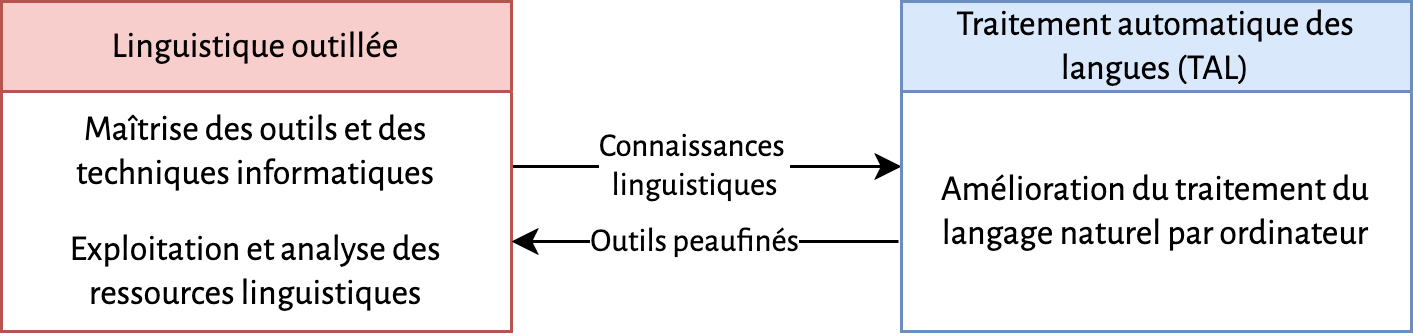
\includegraphics[width=\linewidth]{img/linguistique_outillee_TAL.png}
	\caption{Adapté de \textcite{hodac}.}
	\label{fig:ling_out_TAL}
\end{figure}


\end{frame}



\begin{frame}{\og{}\textit{Un corpus ne se lit pas, il s'interroge}\fg{}}
	\begin{block}{Corpus électronique}
		\justifying
		Ensemble de données linguistiques (textes écrits ou retranscriptions de discours oraux) rassemblées en un seul et même endroit, qui peut être interrogé automatiquement via une interface en ligne ou via un programme informatique hors ligne (concordancier).


	\end{block}
		\begin{itemize}
		\item échantillon représentatif d’une (variante de) langue
		\begin{itemize}
			\item  variante géographique ; registre, domaine de spécialité$\dots$
		\end{itemize}
		\item peut être associé à d’autres corpus à des fins de comparaison
		\item données brutes (le corpus ne contient que le texte) 
		\item données annotées (corpus étiqueté). 
	\end{itemize}
\begin{flushright}
\citep{loock2017web}
\end{flushright}
\end{frame}

\begin{frame}{Linguistique outillée}
	Outils d'analyse linguistique des corpus de textes :
	        \begin{itemize}
			        	\item concordancier
			        	\item logiciel de textométrie
			        	\item plateforme d'interrogation de corpus
			        \end{itemize}
	Thématiques centrales :		        
			    \begin{itemize}
			    	\item Apport des corpus en sciences du langage
			    	\item Manipulation de corpus : observation de contextes, analyses quantitatives, textométrie, projection de lexiques et de patrons
			    	\item Diversité des corpus
			    	\item Études linguistiques outillées d’un corpus diversifié
			        \end{itemize}
			        
\end{frame}

\begin{frame}{\textsc{TAL}}
	
	{\scriptsize angl. \textit{natural language processing} (\textsc{NLP})}
	
	Thématiques centrales :
	\begin{itemize}
		\item Panorama des techniques et des niveaux d’analyse linguistique
		\item Applications :
		\begin{itemize}
			\item {\small\textsc{OCR}\footnote{\textit{Optical Character Recognition}}} : reconnaissance optique de caractères
			\item {\small\textsc{NER}\footnote{\textit{Named Entity Recognition}}} : reconnaissance d'entités nommées
			\item {\small extraction terminologique}
		\end{itemize}
		\item Programmation (p. ex. en Python)
		\item Outils d'étiquetage et d'analyse morphosyntaxiques 
		\item Évaluation de l’efficacité des outils du \textsc{TAL}
	\end{itemize}
\end{frame}

\begin{frame}{Écosystème}
	\begin{figure}[h] % Use [H] to force the figure to stay in place
		\centering
		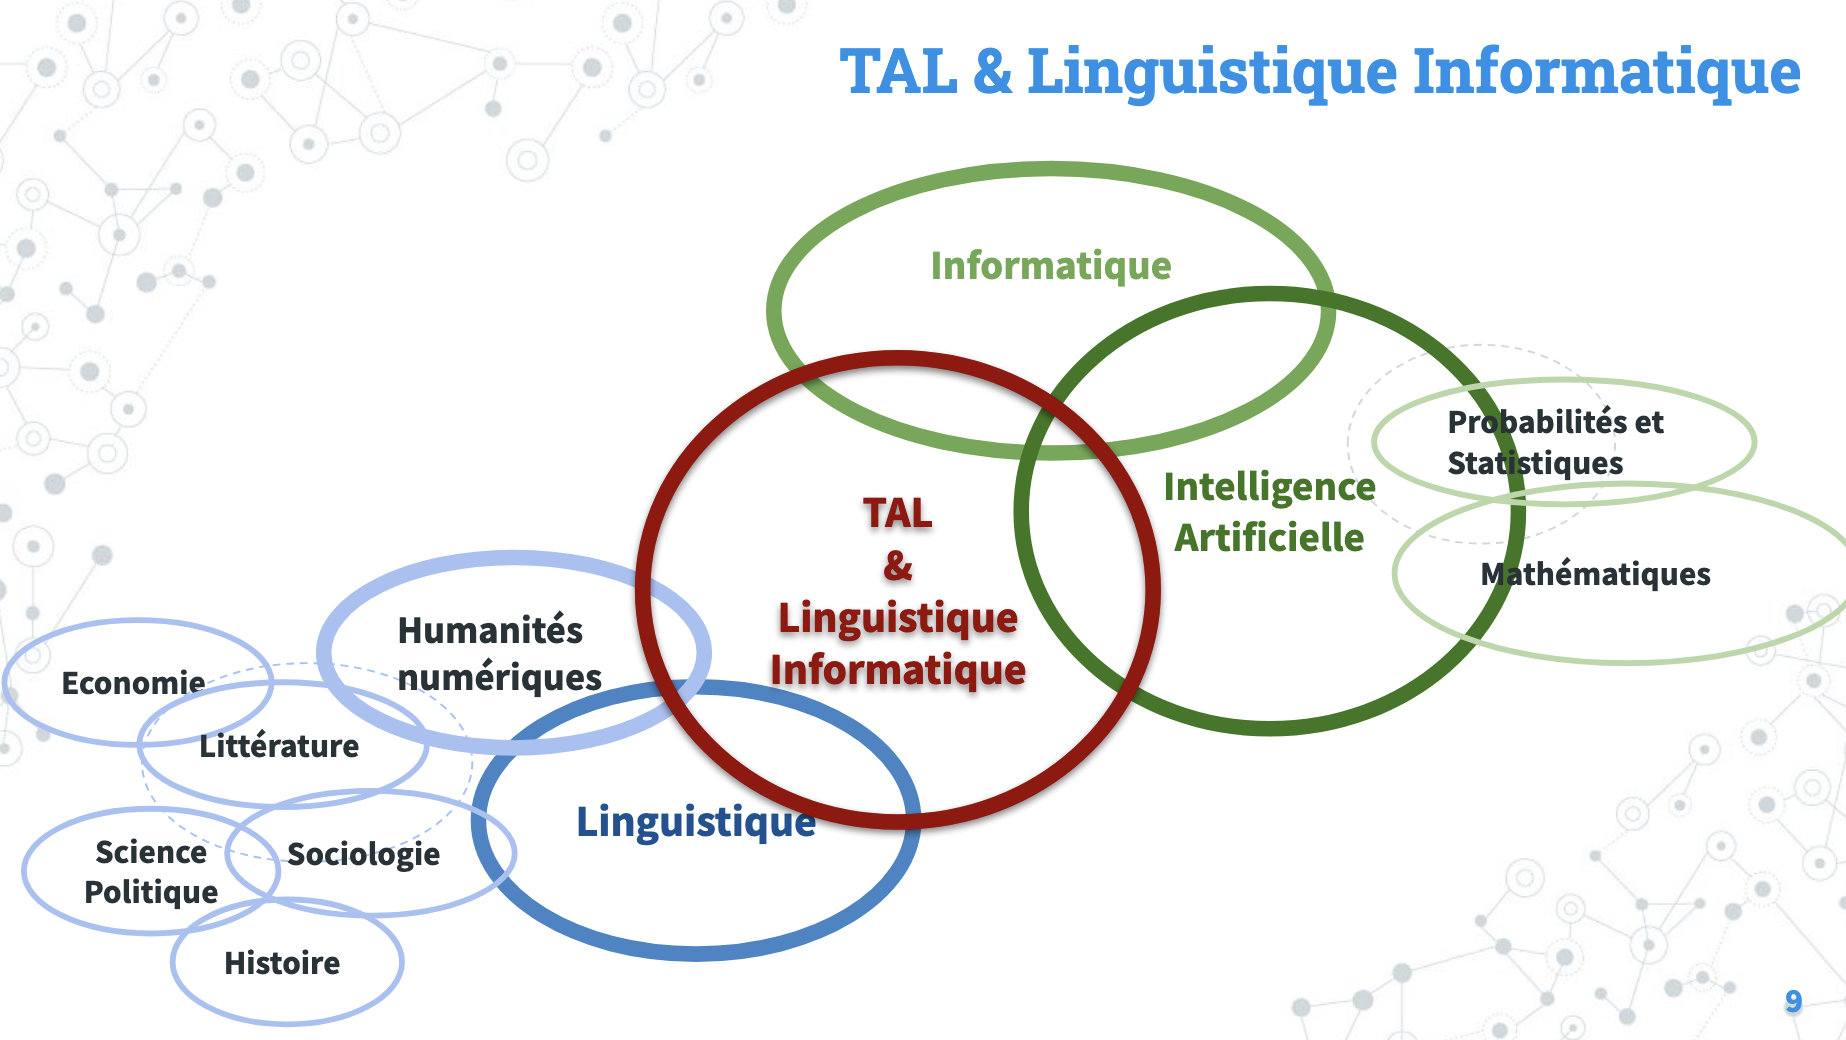
\includegraphics[width=0.80\linewidth]{img/ecosysteme.png}
		%	\caption{}
		\label{fig:ecosysteme}
		\caption{Le \textsc{TAL} et la linguistique informatique dans l'écosystème des sciences \citep{boisson}.}
	\end{figure}
\end{frame}


\section{Fondamentaux du \textsc{TAL}}

\begin{frame}{Envergure}
	\begin{block}{\vspace{-6mm}}
			\justifying
		Domaine de recherche pluridisciplinaire à l'intersection de la linguistique et de l'informatique $\rightarrow$ \textsc{IA}, apprentissage artificiel.
	\end{block}
	\vspace{-4mm}
		\begin{flushright}
		\citep{poibeau}
	\end{flushright}
	
	\begin{block}{\vspace{-6mm}}
			\justifying
	Modéliser et reproduire, à
l’aide de machines, la capacité humaine à
produire et à comprendre des énoncés linguistiques
	\end{block}
	\vspace{-4mm}
		\begin{flushright}
	\citep{yvon2010petite}
\end{flushright}

	\begin{itemize}
		\item analyse (compréhension) des langues
		\item génération de texte
		\item ingénierie linguistique : focus sur les aspects pratiques
		\item linguistique informatique : focus sur la linguistique
	\end{itemize}
\end{frame}

\begin{frame}{Applications}
	
	Liste non exhaustive :
	\begin{itemize}
		\item traduction automatique 
		\item agents conversationnels 
		\item correcteur orthographique
		\item prédiction du prochain mot
		\item classification du texte
		\item annotation morphosyntaxique
	\end{itemize}
	
\end{frame}

\begin{frame}{Évolution du domaine}
\begin{figure}[h] % Use [H] to force the figure to stay in place
	\centering
	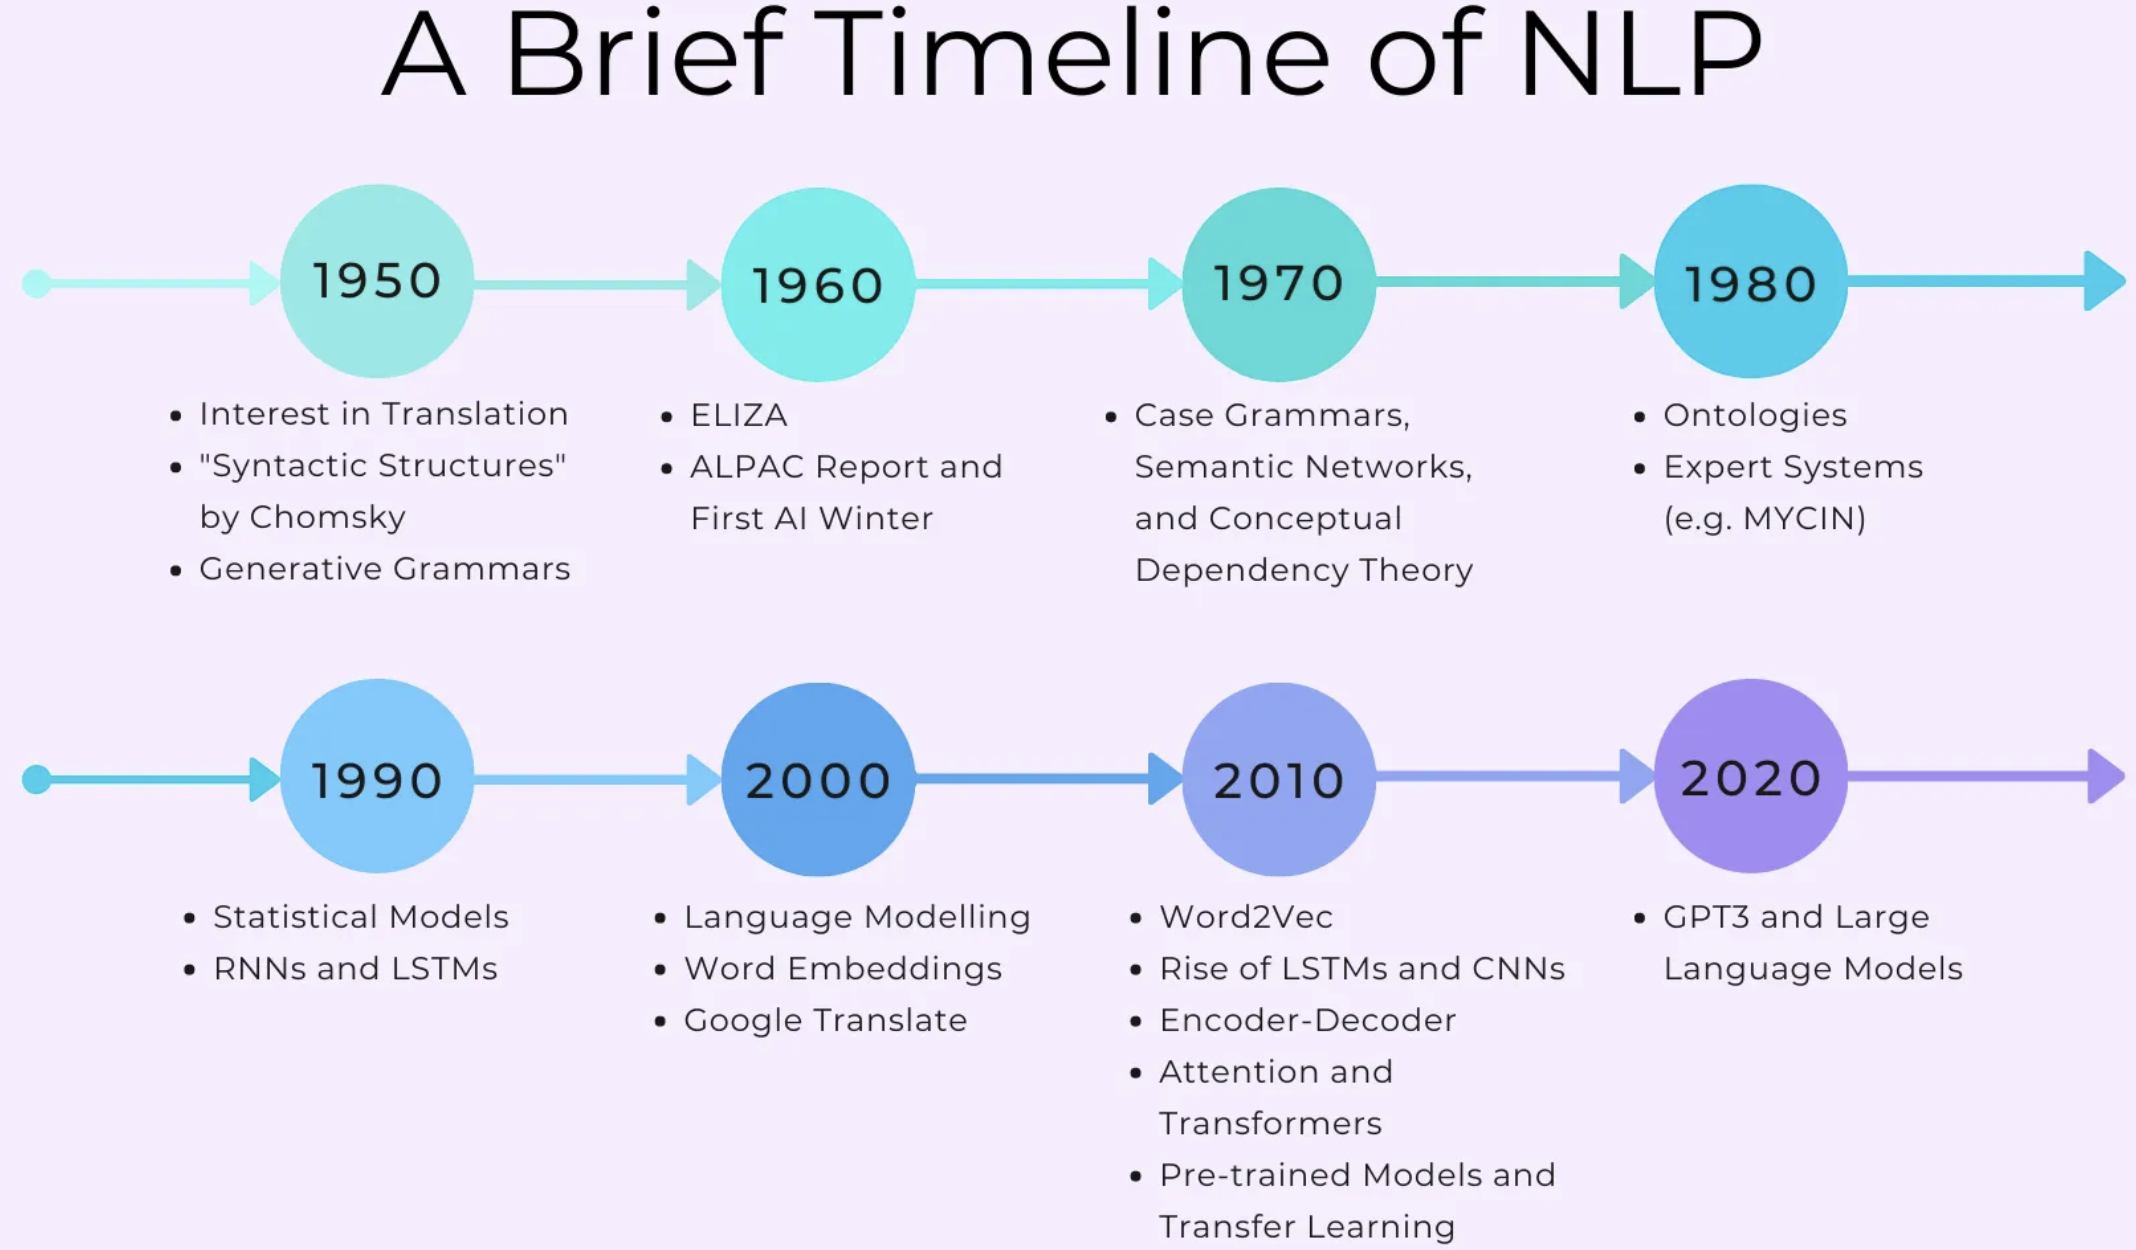
\includegraphics[width=\linewidth]{img/evolution.png}
	%	\caption{}
	\label{fig:evolution}
	\caption{L'histoire du \textsc{TAL} \citep{chiusano2022}.}
\end{figure}

\end{frame}




\begin{frame}{Techniques}
Systèmes à base de \bolder{règles}
\begin{itemize}
	\item construites par un humain (linguiste)
	\item saisie manuelle
\end{itemize} 

Systèmes \bolder{orientés données} (angl. \textit{data-driven})
\begin{itemize}
	\item apprentissage (non) supervisé
	\item à partir d'exemples annotés par un humain
\end{itemize}
\end{frame}

\begin{frame}{Représentations vectorielles}
	Plongements (angl. \textit{embeddings})
	\begin{itemize}
		\item informations linguistiques représentées par des vecteurs de	caractères, de mots, de phrases, de paragraphes, de documents
		\item + : représentations continues, calculs de similarité
		\item - : ne prend pas en compte la polysémie d'un mot
	\end{itemize}

\end{frame}

\begin{frame}{Limite sémantique des plongements statiques}
	Chaque mot a exactement une représentation vectorielle fixe.
	\begin{figure}[h] % Use [H] to force the figure to stay in place
		\centering
		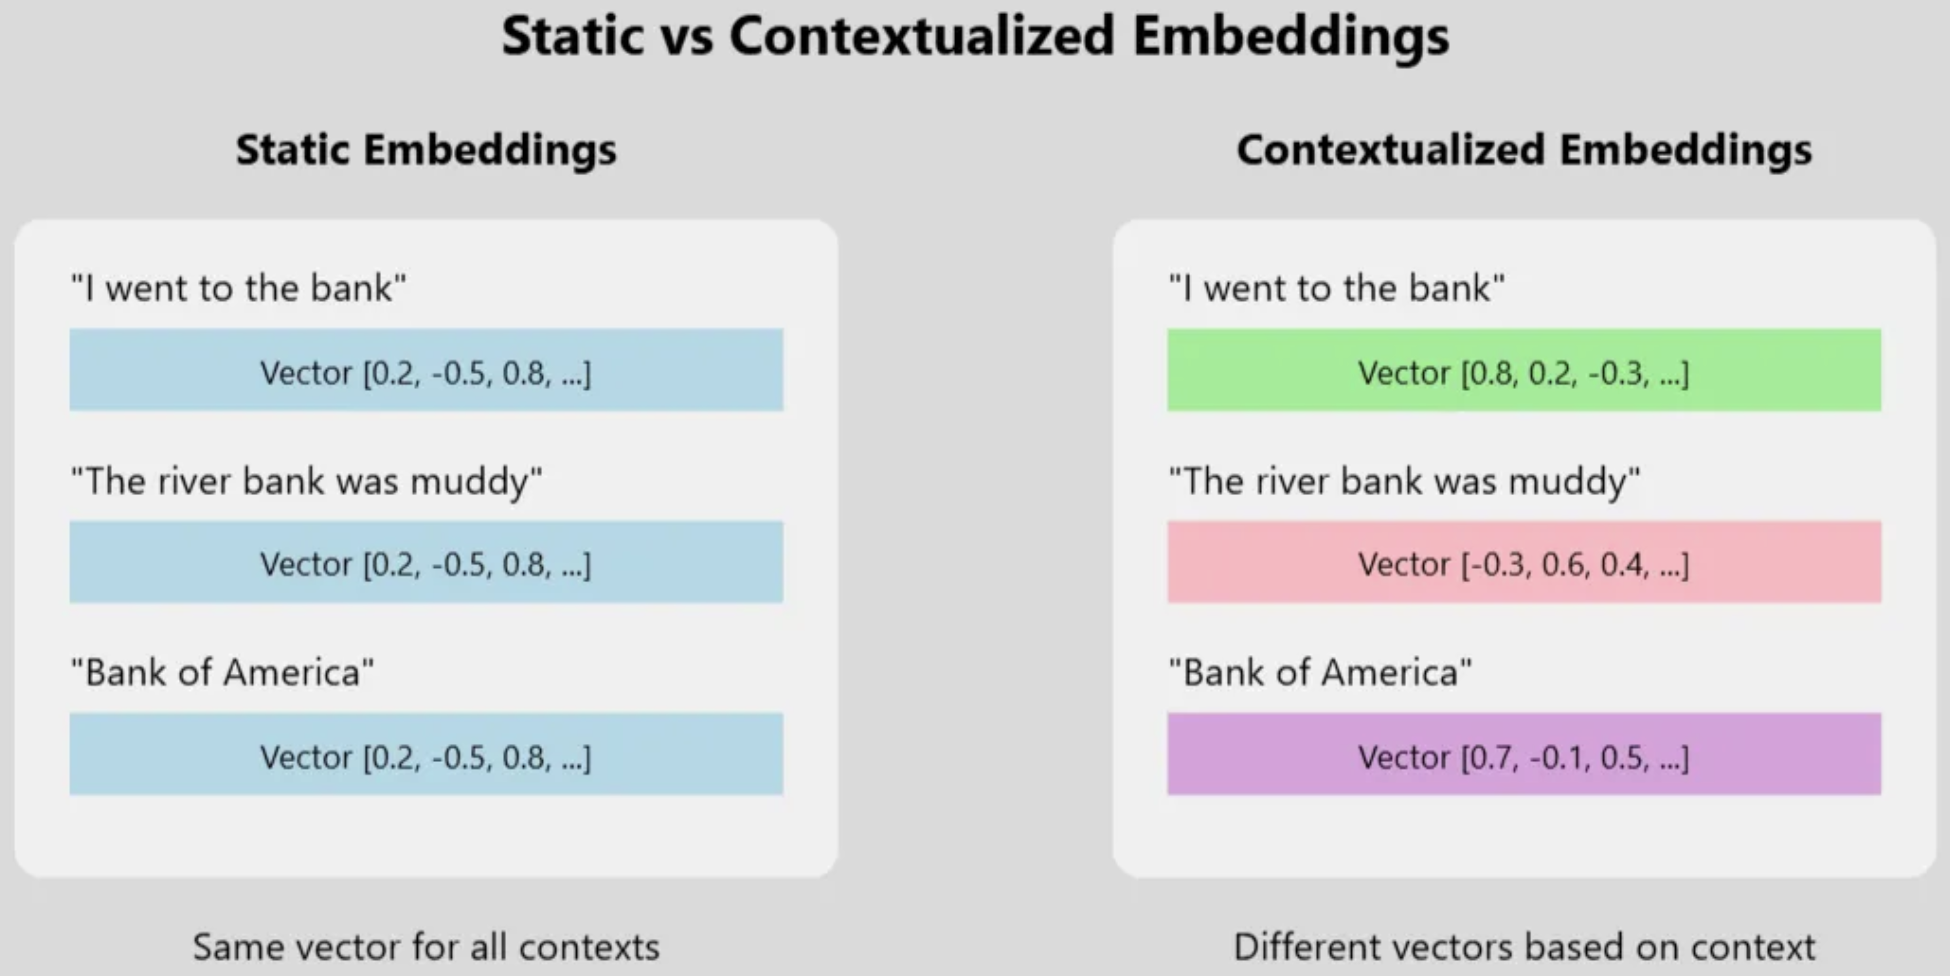
\includegraphics[width=\linewidth]{img/plongements.png}
		%	\caption{}
		\label{fig:plongements}
		\caption{Plongements statiques et contextuels \citep{manikanth2024}.}
	\end{figure}
\end{frame}

\begin{frame}{Modèles de langage}
		\begin{itemize}
		\item doit
		distinguer les séquences (non-)grammaticales
		\item construction d'un modèle de langue statistique permet d'assigner une probabilité à
		une séquence de mots
			\begin{flushright}
			\citep{chomsky1957}
		\end{flushright}
		\begin{itemize}
			\item \og{}je vais à la Sorbonne\fg{} \checkmark
			\item \og{}je à la Sorbonne vais\fg{} \XSolidBrush
		\end{itemize} 
	\end{itemize}

\end{frame}

\begin{frame}{Modèles de langage : apprentissage à partir des
		données}
	\bolder{Entraînement}
	\begin{itemize}
		\item non supervisé (pré-entraînement) :
		\begin{itemize}
			\item  apprentissage à partir des grands corpus de textes
		\end{itemize} 
		\item supervisé (\textit{fine-tuning})
		\begin{itemize}
			\item annotation des données pour une tâche spécifique \item spécialisation du modèle
			\item le modèle reçoit l'\textit{input} et l'\textit{output} correct
			\item il apprend à partir d'exemples
			\item p. ex. \textsc{REN} : Marie $\rightarrow$ \textit{Marie} \texttt{[PER]}
		\end{itemize}  
	\end{itemize}
	\bolder{Prédiction}
	
	Le modèle prédit le résultats sur des données non vues.
	
\end{frame}

\begin{frame}{État de l'art : apprentissage profond}
	
	{\scriptsize angl. \textit{\textit{\textbf{D}eep \textbf{L}earning}}}
	
	\begin{itemize}
		\item techniques inspirées par les réseaux de neurones biologiques
		\item des informations très riches associées aux mots 
		\item modélisation des passages textuels entiers (phrase, §)
		\item grands modèles de langage : \textsc{BERT}, ...\textsc{GPT4}
		\item gourmandes en ressources, exigent une puissance de calcul
		\item introduit des biais : racisme, sexisme etc.
		\item langues dotées (français) et peu dotées (quechua)
	\end{itemize}
	
	
	
\end{frame}

\begin{frame}{Ambiguïté}
\begin{block}{\vspace{-6mm}}
	Comment traiter informatiquement l'ambiguïté du langage ?
\end{block}

Ambiguïté \textbf{lexicale}

\begin{itemize}
	\item Ambiguïté catégorielle :
	\begin{itemize}
		\item la \underline{ferme} (\texttt{N})
		\item je \underline{ferme} (\texttt{V})
	\end{itemize}
	\item Polysémie :
	\begin{itemize}
		\item \underline{roi} de France
		\item \underline{roi} de la jungle
	\end{itemize}
\end{itemize}



Ambiguïté \textbf{syntaxique} et \textbf{résolution de coréférence}
\begin{itemize}
	\item Fabrice regarde [Laetitia] [avec \underline{son} télescope].
\end{itemize}
%	\textit{La belle porte le voile.}
%	
%	\begin{itemize}
%		\item la belle (nom, sujet)  ferme (v. \og{}fermer\fg{})  le voile (nom, \textsc{COD}).
%		\item
%		la belle (adj.)  ferme (nom, sujet)  le voile (v. \og{}voiler\fg{}). 
%	\end{itemize}
\end{frame}

\begin{frame}{Segmentation en mots}
	
	\begin{block}{Tokenisation}
			Transformation d'un texte en une série de \textit{tokens} individuels.
	\end{block}

	Un token représente un mot.
	
	 Découpage en tokens (segmentation) :
	\begin{itemize}
		\item \textit{J’ai froid} $\rightarrow$ \texttt{J'} + \texttt{ai} + \texttt{froid}
		\item \textit{aujourd'hui} $\rightarrow$ \texttt{aujourd'hui}
	\end{itemize}
	 Séparateurs : espace, virgule, nouvelle ligne, tab., apostrophes$\dots$
	
	
\end{frame}

\begin{frame}{Tokenisation}
	\begin{figure}[h] % Use [H] to force the figure to stay in place
		\centering
		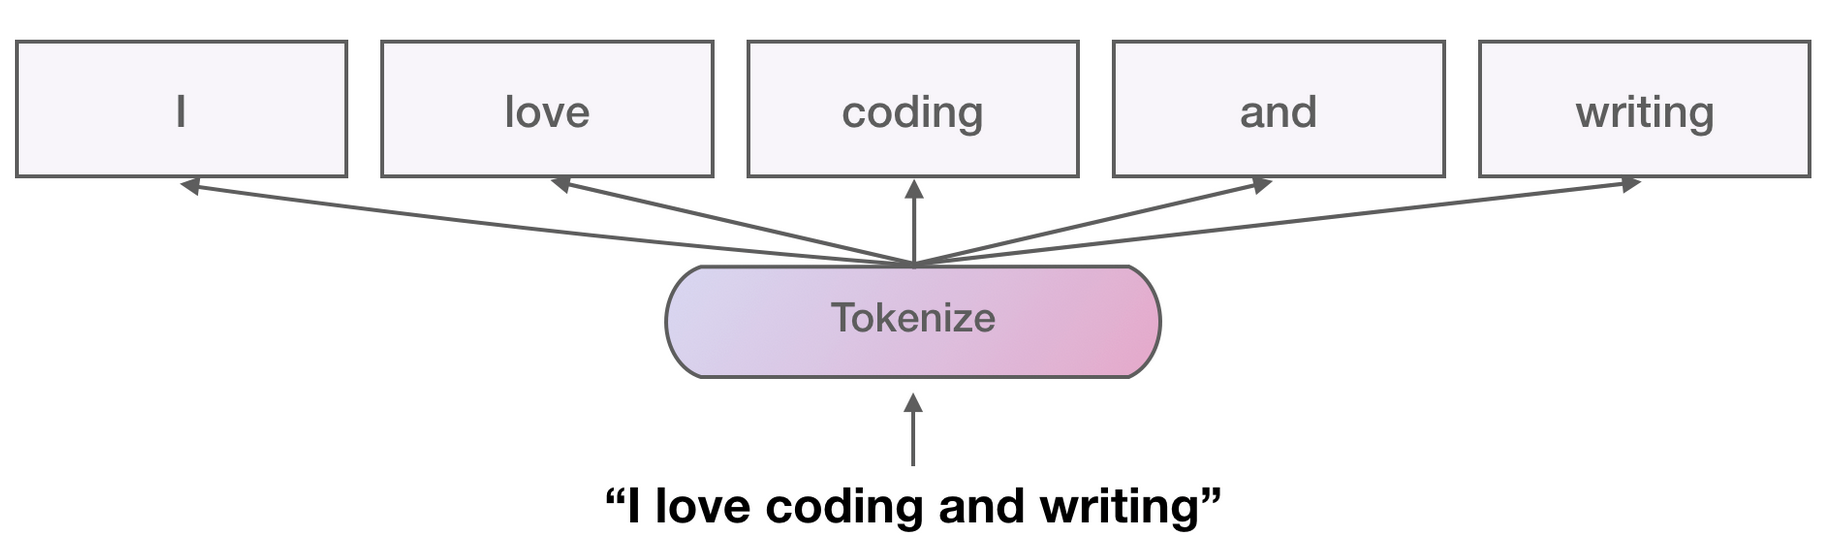
\includegraphics[width=\linewidth]{img/tokenisation.png}
		%	\caption{}
		\label{fig:evolution}
		\caption{Exemple de tokenisation \citep{saravia}.}
	\end{figure}
\end{frame}

\begin{frame}{Segmentation en phrases}
	\begin{itemize}
		\item se termine par une ponctuation de fin de phrase : \texttt{. ; ? !}
		\item la phrase suivante commence par une espace ou un retour à la ligne suivi d’une majuscule
		\item les . . . forment une ponctuation unique
	\end{itemize}
		\begin{figure}[h] % Use [H] to force the figure to stay in place
		\centering
		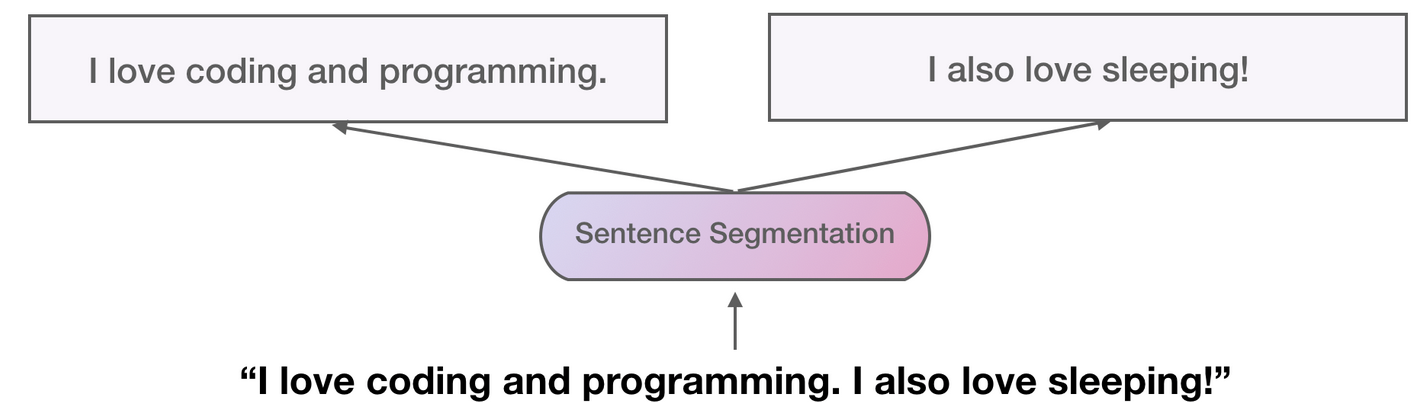
\includegraphics[width=\linewidth]{img/segmentation_phrases.png}
		%	\caption{}
		\label{fig:evolution}
		\caption{Exemple de la segmentation en phrases \citep{saravia}.}
	\end{figure}
\end{frame}

\begin{frame}{Lemmatisation}
\begin{block}{\vspace{-6mm}}
	\justifying
	Réduction des différentes formes d’un mot à une forme canonique : \textit{lemme}.
\end{block}
	\begin{figure}[h] % Use [H] to force the figure to stay in place
	\centering
	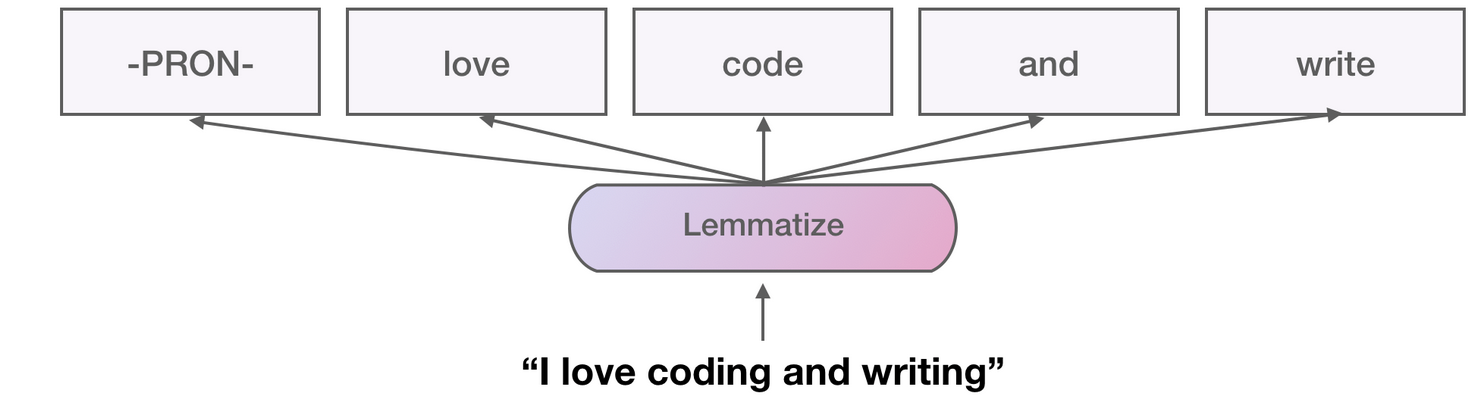
\includegraphics[width=\linewidth]{img/lemmatisation.png}
	%	\caption{}
	\label{fig:evolution}
	\caption{Exemple de lemmatisation \citep{saravia}.}
\end{figure}
\end{frame}

\begin{frame}{Racinisation}
	{\scriptsize angl. \textit{steming}}
	\begin{block}{\vspace{-6mm}}
		\justifying
	Remplacement d'un mot par sa racine morphologique (\textit{radical}).
	\end{block}
		\begin{figure}[h] % Use [H] to force the figure to stay in place
		\centering
		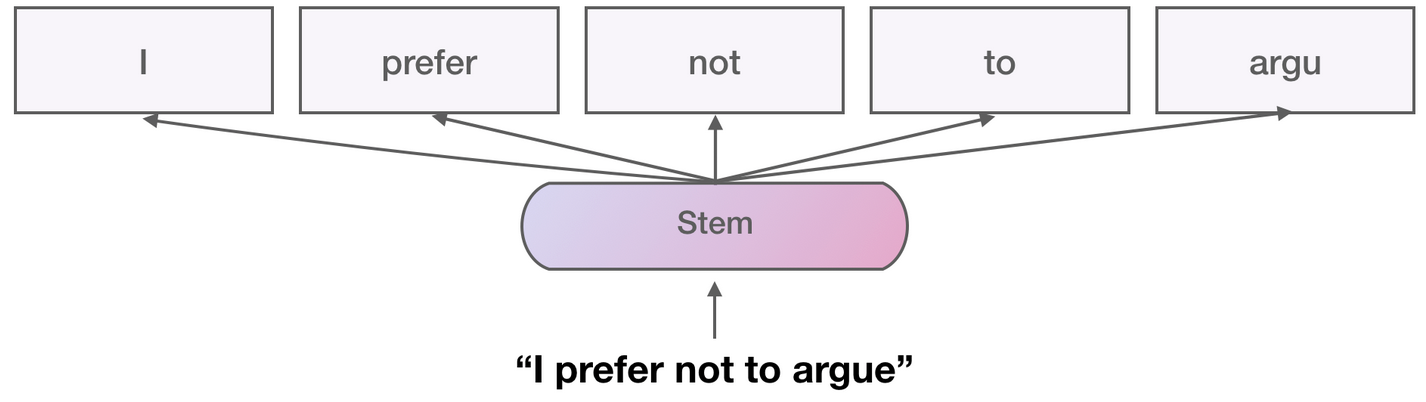
\includegraphics[width=\linewidth]{img/racinisation.png}
		%	\caption{}
		\label{fig:racinisation}
		\caption{Exemple de racinisation \citep{saravia}.}
	\end{figure}
\end{frame}

\begin{frame}{Étiquetage morphosyntaxique}
	\begin{block}{\vspace{-6mm}}
		\justifying
		Assigner des informations grammaticales à chaque mot d’un texte.
	\end{block}
			\begin{figure}[h] % Use [H] to force the figure to stay in place
		\centering
		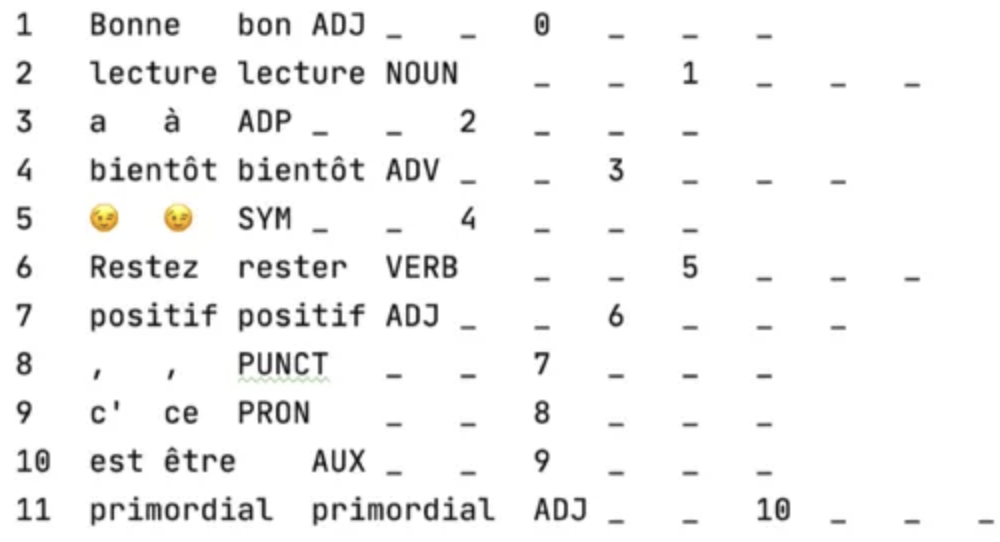
\includegraphics[width=0.80\linewidth]{img/etiquetage.png}
		%	\caption{}
		\label{fig:etiquetage}
		\caption{Exemple d'étiquetage morphosyntaxique \citep{wang2021}.}
	\end{figure}
\end{frame}

\begin{frame}{Évaluation des systèmes de \textsc{TAL}}
	\begin{table}[h]
		\begin{tabular}{ll}
			\bolder{\textbf{P}récision} & \% d'éléments pertinents détectés par le système parmi\\ & tous les éléments détectés\\
			\bolder{\textbf{R}appel} & \% d'éléments pertinents détectés par le système parmi\\ & tous les éléments à détecter\\
			\bolder{\textsc{F}-mesure} & \og{}moyenne harmonique\fg{} de la \textsc{P} et du \textsc{R} ;\\
			& donne le même poids à la \textsc{P} et au \textsc{R} : 
		\end{tabular}
	\end{table}

    \begin{equation*}    % <--- deleted empty lines
	F\text{-}mesure = \frac{2 \times (P \times R)}{P + R}
\end{equation*}
\end{frame}

\begin{frame}{Exemple de l'évaluation}
	Corpus de 100 documents, dont 8 pertinents à la requête.
	
	Le système propose 12 documents, dont 6 pertinents.
	
	$P = \dfrac{6}{12} = 0,5$
	
	$R = \dfrac{6}{8} = 0,75$
	
	\begin{itemize}
		\item \og{}\bolder{bruit}\fg{} : 6 documents proposés à tort
		\item \og{}\bolder{silence}\fg{} : 2 documents \og{}oubliés\fg{} qui auraient dû être détectés, mais ne l'ont pas été
	\end{itemize}
\end{frame}

\begin{frame}{Loi de Zipf}
		\begin{block}{\vspace{-6mm}}
		\justifying
	Dans un corpus d'une langue, la fréquence d'un mot est inversement proportionnelle à son rang dans la liste globale des mots après le tri par ordre décroissant de fréquence.
	\end{block}
	\begin{table}[h]
		\begin{tabular}{|c|c|c|}
			\hline
			\textbf{Rang} & \textbf{Mot} & Fréquence\\
						\hline
			1 & de & 30\\
						\hline
			2 & des & 20\\
						\hline
			$\dots$ &$\dots$ & $\dots$\\
						\hline
			100 & optimisation & 1\\
						\hline
		\end{tabular}
	\end{table}

\end{frame}
\begin{frame}{Visualisation de la loi de Zipf}
	\begin{figure}[h] % Use [H] to force the figure to stay in place
		\centering
		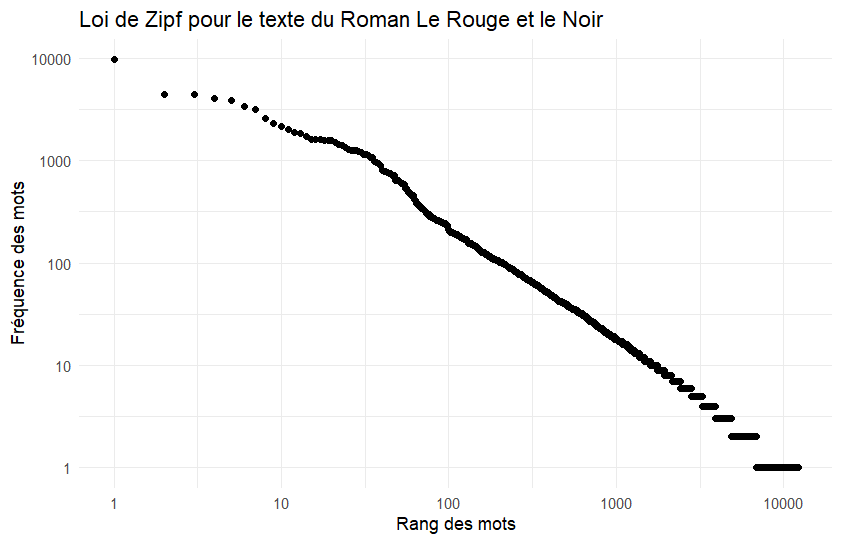
\includegraphics[width=0.80\linewidth]{img/zipf.png}
		\caption{Exemple de la loi de Zipf \citep{rherrad}.}
		\label{fig:zipf}
	\end{figure}
\end{frame}

\begin{frame}{Applications de la loi de Zipf dans la fouille de textes}
			\begin{figure}[h] % Use [H] to force the figure to stay in place
		\centering
		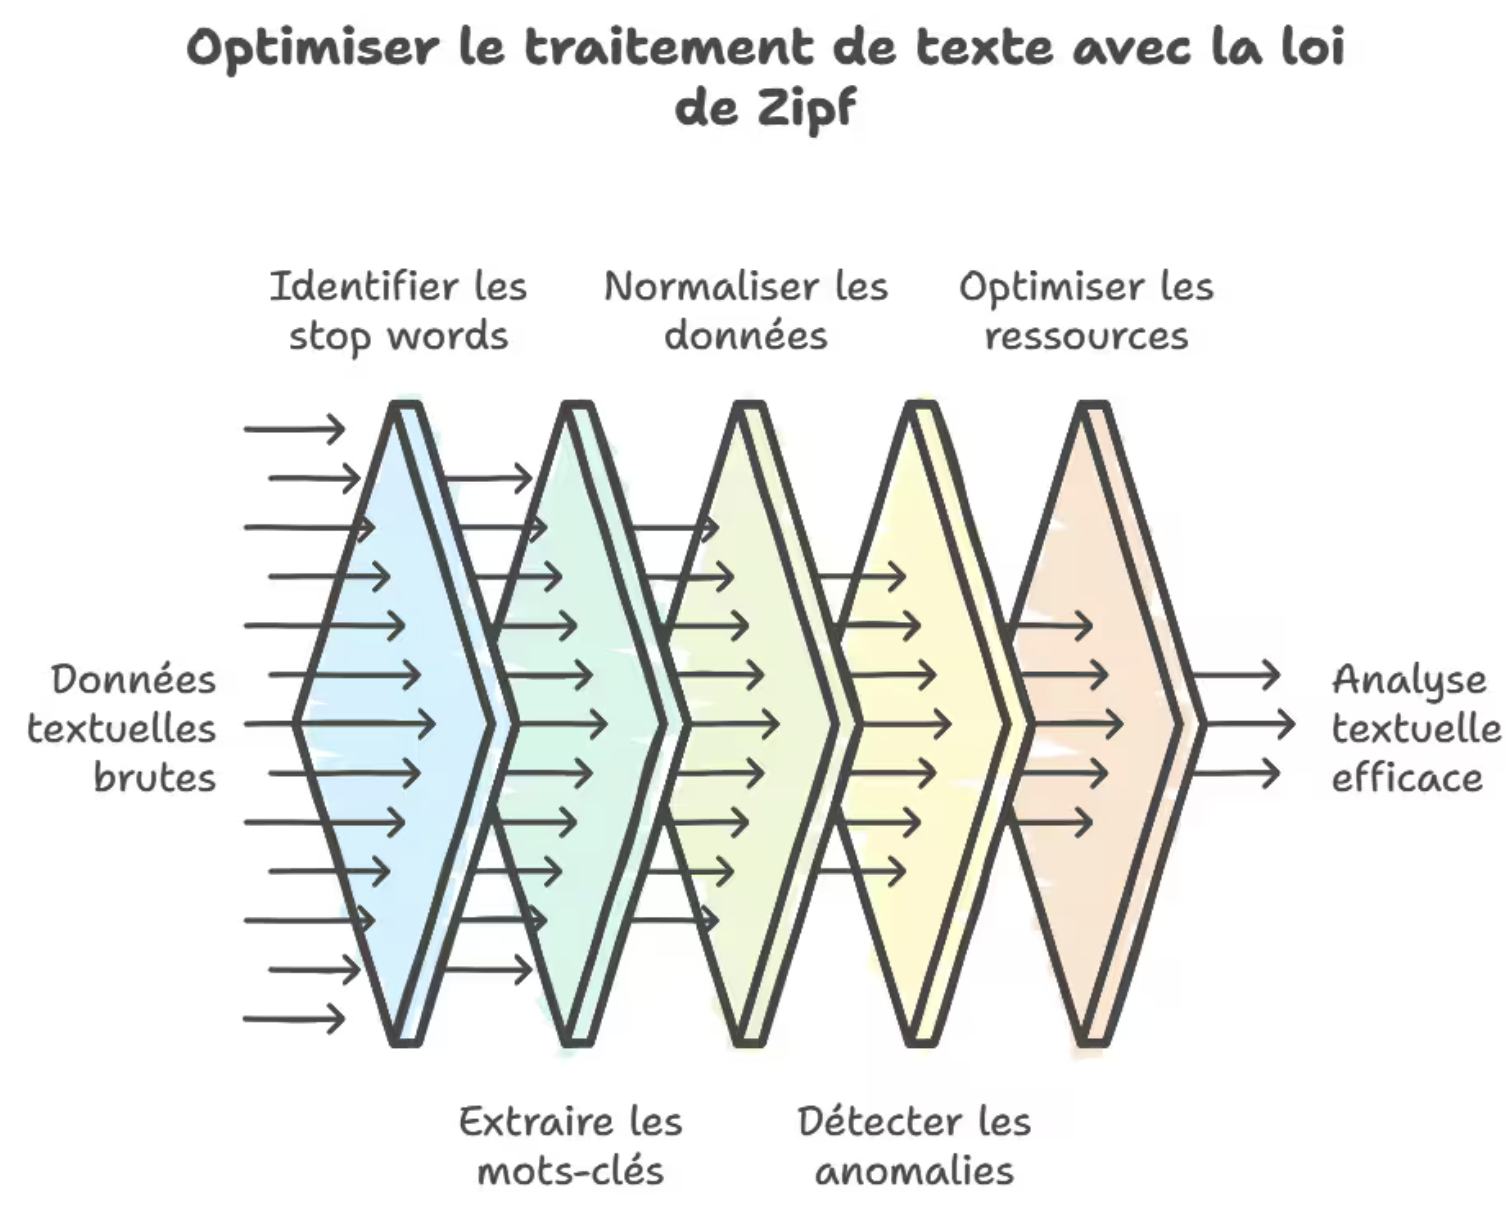
\includegraphics[width=0.80\linewidth]{img/optimisation_zipf.png}
		\caption{Optimisation du traitement du texte avec la loi du Zipf \citep{rherrad}.}
		\label{fig:optimisation_zipf}
	\end{figure}
\end{frame}


\begin{frame}[allowframebreaks]
		\printbibliography
\end{frame}

\end{document}